\chapter{Neighborhood-Based Methods}  
\label{chap:knn}  

One of the simplest and yet often most effective recommender system
methods is based on this natural principle: 

\begin{quote}

Say we have a user U, for whom we want to predict the rating of an item I.
We find the users in our existing data D who are most similar to U and who
have seen rating I, and take our predicted value to be the average of
those users' ratings of I.  

\end{quote}

Note that here the user U might be in D or might be new.  As long as I
is in D, we are in business.

Of course, we must define ``similar.''  There are two common ways to do
this.  Recall our notation $p$ denoting our number of
predctors/features.  This would include our user and item IDs, and
possible covariates.  Then consider these approaches:

\begin{itemize}

\item Define some distance function, and then find the $k$ closest
people in D to U.  

\item Develop a system of rectangles --- hyperrectangles in
$p$-dimensional space --- and determine which one U falls in.  

\end{itemize} 

The first is basically \textit{k-Nearest Neighbor regression} (kNN), a
classic statistics/machine learning technique, though note that a major
difference here is that we only consider users in D who have rated the
same products as N.  

The second can be viewed as something called \textit{kernel regression}, 
but we will add a tree-based structure, with the result termed
\textit{Classification and Regression Analysis} (CART) for a single
tree and \textit{random forests} for a collection of trees.  In the
latter, we create a collection of systems of rectangles and average over
them.\footnote{The terms ``CART'' and ``random forests'' have 
many variations, but we take the terms as generic.}

\section{kNN}

Let's see how kNN works.

\subsection{Notation}

As before, let $A$ denote the ratings matrix.  The element $a_{ij}$ in
row $i$, column $j$, is the rating that user $i$ has given/would give to
item $j$. In the latter case, $a_{ij}$ is unknown, and its predicted value
will be denoted by $\widehat{a}_{ij}$.  Following R notation, we will
refer to the unknown values as NAs.

Note that for large applications, the matrix $A$ is far too large to
store in memory.  One could resort to storage schemes for
\textit{sparse} matrices, e.g.\ \textit{Compresed Row Storage}, but here
we will simply use $A$ to help explain concepts.  In the
\textbf{rectools} package,\footnote{https://github.com/matloff/rectools}
the input data is run through
\textbf{formUserData()} and algorithms use that instead of $A$.  This
function organizes the data into an R list, one element per user.  Each
such element records the ratings made by that user. 

Let's refer to a new case to be predicted as NC, i.e. from above,
predicting how a user U would rate an item I.

\subsection{User-Based Filtering}

In predicting how a given user would rate a given item, we first find
all users that have rated the given item, then determine which of those
users are most similar to the given user.  Our prediction is then the
average of the ratings of the given item among such ``similar'' users.
A corresponding approach based on similar items, \textit{item-based
filtering}, is used as well.  We focus on such methods in this chapter.

% \subsubsection{Matrix View}
% 
% In terms of the matrix $A$ above, we first look at column $j$.  We cull
% the rows having non-NA values in this column, and for each of those
% rows, find the distance of that row to the NC.  Take the $k$ closest
% rows, and finally, average the value of $a_{mj}$ to get
% $\widehat{a}_{ij}$ (with $m$ ranging over the row numbers of the
% selected rows).

\subsection{(One) Implementation}

Below is code from \textbf{rectools} (somewhat
simplified).\footnote{This function was written largely by Vishal
Chakraborti.} The arguments are:

\begin{itemize}

\item \textbf{origData:}  The original dataset, after having been run through
\textbf{formUserData()}. 

\item \textbf{newData:}  The element of \textbf{origData} for NC.\footnote{If
NC is new, not in the database (called \textit{cold start}), we
synthesize a list element for it, assuming NC has rated at least one
item.}

\item \textbf{newItem:}  ID number of the item to be predicted for NC.

\item k:  The number(s) of nearest neighbors.  Can be a vector.

\end{itemize} 

Here is an example of using \textbf{formUserData()} on the MovieLens
data:\footnote{The data have been read from disk without converting to R
factors.}

\begin{lstlisting}
> head(ml)
V1  V2 V3
1 196 242  3
2 186 302  3
3  22 377  1
4 244  51  2
5 166 346  1
6 298 474  4
> mlud <- formUserData(ml)
> mlud[[3]]
$userID
[1] "3"

$itms
[1] 335 245 337 343 323 331 294 332 328 334 350 341 318 300
[15] 345 299 324 348 351 330 327 307 272 354 264 349 321 260
[29] 268 288 355 320 258 339 342 303 329 317 181 338 302 322
[43] 352 271 333 344 326 319 325 347 336 353 340 346

$ratings
335 245 337 343 323 331 294 332 328 334 350 341 318 300 345 
1   1   1   3   2   4   2   1   5   3   3   1   4   2   3 
299 324 348 351 330 327 307 272 354 264 349 321 260 268 288 
3   2   4   3   2   4   3   2   3   2   3   5   4   3   2 
355 320 258 339 342 303 329 317 181 338 302 322 352 271 333 
3   5   2   3   4   3   4   2   4   2   2   3   2   3   2 
344 326 319 325 347 336 353 340 346 
4   2   2   1   5   1   1   5   5 

attr(,"class")
[1] "usrDatum"
\end{lstlisting}

So, for any given user, \textbf{mlud} will show the items rating by this
user and the ratings the user has given to those items.  Here we see
that user 3 has rated items 335, 245,, 337, 343,..., with ratings 1,1,1,3,...

\begin{lstlisting}[numbers=left]
predict.usrData <- function(origData,newData,newItem,k)
{
# we first need to narrow origData down to the users who 
# have rated newItem

# here oneUsr is one user record in origData; the function will look for a 
# j such that element j in the items list for this user matches the item 
# of interest, newItem; (j,rating) will be returned

checkNewItem <- function(oneUsr) {
   whichOne <- which(oneUsr$itms == newItem)
   if (length(whichOne) == 0) {
      return(c(NA,NA))
   } else return(c(whichOne,oneUsr$ratings[whichOne]))
}

found <- as.matrix(sapply(origData,checkNewItem))
# description of 'found':
# found is of dimensions 2 by number of users in training set
# found[1,i] = j means origData[[i]]$itms[j] = newItem;
# found[1,i] = NA means newItem wasn't rated by user i
# found[2,i] = rating in the non-NA case

# we need to get rid of the users who didn't rate newItem
whoHasIt <- which(!is.na(found[1,]))
origDataRatedNI <- origData[whoHasIt]
# now origDataRatedNI only has the relevant users, the ones who 
# have rated newItem, so select only those columns of the found matrix
found <- found[,whoHasIt,drop=FALSE]

# find the distance from newData to one user y of origData; defined for
# use in sapply() below
onecos <- function(y) cosDist(newData,y,wtcovs,wtcats)
cosines <- sapply(origDataRatedNI,onecos)
# the vector cosines contains the distances from newData to all the
# original data points who rated newItem

# action of findKnghbourRtng(): find the mean rating of newItem in
# origDataRatedNI, for ki (= k[i]) neighbors
#
# if ki > neighbours present in the dataset, then the 
# number of neighbours is used
findKnghbourRtng <- function(ki){
  ki <- min(ki, length(cosines))
  # nearby is a vector containing the indices of the ki closest neighbours
  nearby <- order(cosines,decreasing=FALSE)[1:ki]
  mean(as.numeric(found[2, nearby]))
}
sapply(k, findKnghbourRtng)
}
\end{lstlisting}

\subsection{Not Really a Distance}

Note that the distances were computed by the function
\textbf{cosDist()}, which computes a ``cosine'' similarity:

\begin{lstlisting}
find cosine distance between x and y, objects 
# of 'usrData' class 
# 
# only items rated in both x and y are used; if none 
# exist, then return NaN 
# 
#  wtcovs: weight to put on covariates; NULL if no covs 
#  wtcats: weight to put on item categories; NULL if no cats 

cosDist <- function(x,y,wtcovs=NULL,wtcats=NULL) 
{ 
# rated items in common 
commItms <- intersect(x$itms,y$itms) 
if (length(commItms)==0) return(NaN) 
# where are those common items in x and y? 
xwhere <- which(!is.na(match(x$itms,commItms))) 
ywhere <- which(!is.na(match(y$itms,commItms))) 
xvec <- x$ratings[xwhere] 
yvec <- y$ratings[ywhere] 
if (!is.null(wtcovs)) { 
   xvec <- c(xvec,wtcovs*x$cvrs) 
   yvec <- c(yvec,wtcovs*y$cvrs) 
} 
if (!is.null(wtcats)) { 
   xvec <- c(xvec,wtcats*x$cats) 
   yvec <- c(yvec,wtcats*y$cats) 
} 

xvec %*% yvec / (l2a(xvec) * l2a(yvec)) 
}

l2a <- function(x) sqrt(x %*% x) 
\end{lstlisting}

Basically, the ``distance'' between two rows $u$ and $v$
of $A$ is defined by

\begin{equation}
\frac{u'v}{||u||_2 ~ ||v||_2}
\end{equation}

This not really a distance,\footnote{IN math terms, it's not a
\textit{metric}.} but it is a common measure of similarity between two
vectors in machine learning.  In two or three dimensions, it really is
the cosine of the angle between $u$ and $v$.  

Note that larger cosines mean the vectors are more similar.  We find the
$k$ most similar rows in D to U, and average their ratings of the given
item.

\subsection{Regression Analog}

Recall the method of k-nearest neighbor (kNN) regression estimation from
Chapter \ref{chap:infra2}, involving prediction of weight from height
and age:

\begin{quote}
To estimate $E(W ~| H=70, A=28)$, we could find, say, the 25 people in our
sample for whom $(H,A)$ is closest to (70,28), and average their weights
to produce our estimate of $E(W ~| H=70, A=28)$.
\end{quote}

So kNN RS is really the same as kNN regression

\subsection{Choosing k}

As we have already seen with RS, regression and machine learning methods, 
the typical way to choose a model is to use cross-validation.  This is
true for kNN RS as well; we can choose the value of $k$ via
cross-validation.  

% However, a curious property may streamline the process, as follows.
% 
% Note this line in \textbf{predict.usrData()}:
% 
% \begin{lstlisting}
% ki <- min(ki, length(cosines))
% \end{lstlisting}
% 
% What is happening here?  Say for a particular situation, there are 52
% rows in $A$ having ratings for the item specified in NC.  Then of course
% as we increase our number of nearest neighbors beyond 52, we will get
% identical results.  Such a situation will occur if the $A$ matrix is not
% too \textit{dense}, i.e.\ does not have a high proportion of non-NA
% values.  

\subsection{Item-Based Filtering}

Consider again our setting in which we wish to predict the rating user U
would give to item I.  We could switch the above procedure, trading rows
for columns.  We would find the columns corresponding to items U has
rated, then find the closest $k$ of those columns to column I.  The
ratings given by U in those closest column would then be averaged to
yield our prediction.

\subsection{Covariates}

To accommodate covariates, we simply add covariate columns to the input
matrix, say now with columns 'userId', 'itemId', 'rating' and age'.

\section{CART and Random Forests}

\iffalse

ml <- read.table('u.data')
userMeans <- tapply(ml$V3,ml$V1,mean)
itemMeans <- tapply(ml$V3,ml$V2,mean)
mlemb <- ml
mlemb$V1 <- userMeans[ml$V2]
mlemb$V2 <- itemMeans[ml$V2]
mlemb$V1 <- as.vector(mlemb$V1)
mlemb$V2 <- itemMeans[ml$V2]
mlemb$V2 <- as.vector(mlemb$V2)
library(partykit)
ctout <- ctree(V3 ~ .,data=mlemb)
# how would user 22 like movie 88?
predict(ctout,data.frame(V1=userMeans[22],V2=itemMeans[88]))
#            V3
# [1,] 3.54066 

\fi

CART is based on forming a \textit{recursive partitioning}

\subsection{Motivating Example}

Let's illustrate CART with the R package \textbf{partykit}.\footnote{The
name is an allusion to the recursive partioning nature of CART.}  We'll
predict weight from height and age in the baseball player data.

\begin{lstlisting}
> library(regtools) 
> data(mlb) 
> mlb <- mlb[,c(4:6)] 
> head(mlb)
  Height Weight   Age
1     74    180 22.99
2     74    215 34.69
3     72    210 30.78
4     72    210 35.43
5     73    188 35.71
6     69    176 29.39
> ctout <- ctree(Weight ~ .,data=mlb) 
\end{lstlisting}

Here is the tree that is produced:

\begin{lstlisting}
> node_party(ctout) 
[1] root
|   [2] V2 <= 73
|   |   [3] V2 <= 70
|   |   |   [4] V3 <= 29.56 *
|   |   |   [5] V3 > 29.56 *
|   |   [6] V2 > 70
|   |   |   [7] V3 <= 32.51
|   |   |   |   [8] V2 <= 72 *
|   |   |   |   [9] V2 > 72 *
|   |   |   [10] V3 > 32.51 *
|   [11] V2 > 73
|   |   [12] V2 <= 75
|   |   |   [13] V3 <= 27.55
|   |   |   |   [14] V2 <= 74 *
|   |   |   |   [15] V2 > 74 *
|   |   |   [16] V3 > 27.55 *
|   |   [17] V2 > 75
|   |   |   [18] V2 <= 79
|   |   |   |   [19] V3 <= 26.03 *
|   |   |   |   [20] V3 > 26.03 *
|   |   |   [21] V2 > 79 *
\end{lstlisting}

We'll look more at the tree shortly, but first suppose we wish to
predict the weight of a player who is 72 inches tall, age 31.

\begin{lstlisting}
> predict(ctout,data.frame(Height=72,Age=31))
       1 
189.9091 
\end{lstlisting}

Where did that come from?  Look at the tree.  Height $\leq$ 73?  Yes, so
go to node 3.  Height $\leq$ 70?  No, go to node 6, etc., winding up at
node 8.  The asterisk indicates a leaf node, so we're done traversing
the tree.` No, what is the mean weight in that node?

\begin{lstlisting}
> ht <- mlb$Height
> age <- mlb$Age
> mean(mlb[70 < ht & ht <= 72 & age <= 32.51,]$Weight)
[1] 189.9091
\end{lstlisting}

\subsection{Use in Recommender Systems}

Clearly, it would be difficult to use CART directly on, say, the
MovieLens data.  Since the user and item IDs are not \textit{ordinal},
i.e.\ do not have an inherent underlying ordering, we'd need to form
dummy variables, and thus test for one of them at a time.  The tree
would be greatly unbalanced, to the right, and we'd have a computational
problem, at the least.

But actually, it's a lot worse than that.  Think of a node ``User ID =
168?''  In cases where we take the left branch, i.e.\ the data point is
indeed for user 168, the next question might be, say, Item ID = 12''?
The key point is that \textbf{there will be at most 1 data point
satisfying both conditions.}   That's not enough to make a good tree.
And indeed, CART software typically sets a minimum node size as a
hyperparameter; for \textbf{ctree(), it's \textbf{minsplit}}.

An alternative is to do an \textit{embedding} of the user and item ID
data, a form of dimension reduction.  What we could do here is replace
each user ID by the mean rating given by that user, and do the same for
the movies:

\begin{lstlisting}

> userMeans <- tapply(ml$V3,ml$V1,mean) 
> itemMeans <- tapply(ml$V3,ml$V2,mean) 
> mlemb <- mlb
> mlemb$V1 <- userMeans[ml$V2]
> mlemb$V2 <- itemMeans[ml$V2]
> mlemb$V1 <- as.vector(mlemb$V1)
> mlemb$V2 <- itemMeans[ml$V2]
> mlemb$V2 <- as.vector(mlemb$V2)
> ctout <- ctree(V3 ~ .,data=mlemb)

\end{lstlisting}

We could then use \textbf{predict()} as before.

PICTURE IS WITH maxdepth = 3
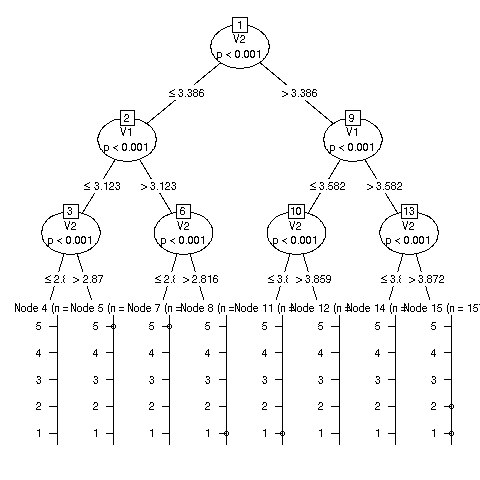
\includegraphics[width=4.2in]{Images/MLmaxdepth3.png}

\subsection{Tuning Parameters}

\subsection{Covariates}

\iffalse 

ml <- read.table('~/tmp/ml-100k/u.data')
ml$V4 <- NULL

idxs <- sample(1:nrow(ml),1000)
ml <- ml[,1:3]
mltrn <- ml[-idxs,]
mltst <- ml[idxs,]
library(rectools)
ud <- formUserData(mltrn)

k <- 5
z <- apply(mltst[,-3],1,pn); mean(abs(z-mltst[,3]),na.rm=T)

predname <- function(userData,oneInputRow,k)
{
   usr <- oneInputRow[1]
   itm <- oneInputRow[2]
   udElement <- userData[[as.character(usr)]]
   predict(userData,udElement,itm,k)
}

pn <- function(oneInputRow) predname(ud,oneInputRow,k)

\fi

